% --------------------------------------------------------------
% This is all preamble stuff that you don't have to worry about.
% Head down to where it says "Start here"
% --------------------------------------------------------------

\documentclass[11pt]{article}

\usepackage[margin=1in]{geometry}
\usepackage{times}
\usepackage{amsmath,amsthm,amssymb}
\usepackage{caption}
\usepackage{graphicx,subfigure}
\usepackage{listings}
\usepackage{url}
\lstset{language=Pascal}

\newcommand{\N}{\mathbb{N}}
\newcommand{\Gauss}{\mathcal{N}}
\newcommand{\Z}{\mathbb{Z}}
\newcommand{\E}{\mathbb{E}}
\newcommand{\R}{\mathbb{R}}
\newcommand{\p}{{\bf p}}
\newcommand{\1}{\mathbf{1}}

\linespread{0}

\newenvironment{theorem}[2][Theorem]{\begin{trivlist}
\item[\hskip \labelsep {\bfseries #1}\hskip \labelsep {\bfseries #2.}]}{\end{trivlist}}
\newenvironment{lemma}[2][Lemma]{\begin{trivlist}
\item[\hskip \labelsep {\bfseries #1}\hskip \labelsep {\bfseries #2.}]}{\end{trivlist}}
\newenvironment{claim}[2][Claim]{\begin{trivlist}
\item[\hskip \labelsep {\bfseries #1}\hskip \labelsep {\bfseries #2.}]}{\end{trivlist}}
\newenvironment{exercise}[2][Exercise]{\begin{trivlist}
\item[\hskip \labelsep {\bfseries #1}\hskip \labelsep {\bfseries #2.}]}{\end{trivlist}}
\newenvironment{problem}[2][Problem]{\begin{trivlist}
\item[\hskip \labelsep {\bfseries #1}\hskip \labelsep {\bfseries #2.}]}{\end{trivlist}}
\newenvironment{question}[2][Question]{\begin{trivlist}
\item[\hskip \labelsep {\bfseries #1}\hskip \labelsep {\bfseries #2.}]}{\end{trivlist}}
\newenvironment{corollary}[2][Corollary]{\begin{trivlist}
\item[\hskip \labelsep {\bfseries #1}\hskip \labelsep {\bfseries #2.}]}{\end{trivlist}}

\begin{document}

% --------------------------------------------------------------
%                         Start here
% --------------------------------------------------------------

\title{ECE 544NA HW1}%replace X with the appropriate number
\author{Jiaqi Mu~jiaqimu2 \\ [8pt]%replace with your name
Department of Electrical and Computer Engineering} %if necessary, replace with your course title

\maketitle

\section{Pencil-and-Paper\label{sec:1}}
Suppose that you have a one-layer neural network, of the form $y_i = g(w'x_i + b)$, where $g()$ is some nonlinearity, $b$ is a trainable scalar bias parameter, and $w'x_i$ means the dot product between the trainable weight vector, $w$, and the $i$-th training vector, $x_i$. Suppose you have a training corpus of the form $D=\{(x_1, t_1), ... , (x_n, t_n)\}$. Turn in your derivations of the following 5 things.

\begin{itemize}
  \item Find the derivatives of $\frac{dE}{dw_j}$ and $\frac{dE}{db}$, where $E=\sum_i ((t_i-y_i)^2)$. Your answer should include the derivative of the nonlinearity, $g'(w'x_i+b)$.
  \begin{proof}
    The derivatives are as follows,
    \begin{align*}
      \frac{dE}{dw_j} &= \sum_i \frac{d}{dw_j}(t_i-y_i)^2 \\
      &= \sum_i 2(t_i-y_i)\frac{d}{dw_j}(t_i-y_i) \\
      &= \sum_i 2(t_i-y_i)(-\frac{dy_i}{dw_j}) \\
      &= \sum_i 2(y_i-t_i)g'(w'x_i + b)x_{ij}, \\
      \frac{dE}{db} &= \sum_i \frac{d}{db}(t_i-y_i)^2 \\
      &= \sum_i 2(t_i-y_i)\frac{d}{b}(t_i-y_i) \\
      &= \sum_i 2(t_i-y_i)(-\frac{dy_i}{db}) \\
      &= \sum_i 2(y_i-t_i)g'(w'x_i + b), \\
    \end{align*}
    where $x_{ij}$ is the $j$-th element of $x_i$.
  \end{proof}
  \item Suppose $g(a) = a$, write $\frac{dE}{dw_j}$ without $g'()$.
  \begin{proof}
    Given that $g(a) = a$, we know $g'(a) = 1$, and therefore the derivatives are,
    \begin{align*}
      \frac{dE}{dw_j} = \sum_i 2(y_i-t_i)x_{ij}.
    \end{align*}
  \end{proof}
  \item Suppose $g(a) = \frac{1}{1+\exp(-a)}$. In this case, $g'(w'x_i+b)$ can be written as a simple function of $y_i$. Write it that way,
  \begin{proof}
    Since $g(a)$ is the logistic function, we can compute $g'(a)$ by,
    \begin{align*}
      g'(a) = -\frac{-\exp(-a)}{(1+\exp(-a))^2} = \frac{1}{1+\exp(-a)}\frac{\exp(-a)}{1+\exp(-a)} = g(a)(1-g(a)).
    \end{align*}
    Thus one can simplify $g'(w'x_i + b)$ by,
    \begin{align*}
      g'(w'x_i + b) = g(w'x_i + b)(1-g(w'x_i + b)) = y_i(1-y_i).
    \end{align*}
  \end{proof}
  \item Use the perceptron error instead: $E = \sum_i \max(0, -(w'x_i+b)\cdot t_i)$.
  \begin{proof}
    The derivatives are as follows,
    \begin{align*}
      \frac{dE}{dw_j} &= \sum_i \dfrac{d}{dw_j} \max(0, -(w'x_i+b)\cdot t_i)  \\ 
      &= \sum_i \1_{t_i(w'x_i + b) < 0} \frac{d}{dw_j} (-w'x_i + b)\cdot t_i \\
      &= \sum_i - \1_{t_i (w'x_i + b < 0)} t_ix_{ij} \\
      \frac{dE}{db} &= \sum_i \dfrac{d}{db} \max(0, -(w'x_i+b)\cdot t_i)  \\ 
      &= \sum_i \1_{t_i(w'x_i + b) < 0} \frac{d}{db} (-w'x_i + b)\cdot t_i \\
      &= \sum_i - \1_{t_i (w'x_i + b < 0)} t_i
    \end{align*}
  \end{proof}
  \item Use the SVM error instead: $E = \|w\|_2^2 +C\sum_i h(x_i, t_i)$, where $h(x_i, t_i) = \max(0, 1-t_i(w'x_i+b))$ is the hinge loss, $C$ is an arbitrary constant, and you can assume that $t_i$ is either $+/-$1.
  \begin{proof}
    The derivatives are as follows,
    \begin{align*}
      \frac{dE}{dw_j} &= \frac{d}{dw_j}\|w\|_2^2 + C\sum_i \frac{d}{dw_j} \max(0, 1-t_i(w'x_i + b))\\
      &= 2w_j + C\sum_i \1_{t_i(w'x_i+b) < 1} \frac{d}{dw_j} (-t_i(w'x_i + b)) \\
      &= 2w_j + C\sum_i -\1_{t_i(w'x_i+b) < 1}x_{ij}t_i, \\
      \frac{dE}{db} &= \frac{d}{db}\|w\|_2^2 + C\sum_i \frac{d}{db} \max(0, 1-t_i(w'x_i + b))\\
      &= C\sum_i \1_{t_i(w'x_i+b) < 1} \frac{d}{db} (-t_i(w'x_i + b)) \\
      &= C\sum_i -\1_{t_i(w'x_i+b) < 1}t_i \\
    \end{align*}
  \end{proof} 
\end{itemize}

\section{Code-From-Scratch}
Write a one-layer neural net that takes a single cepstrum as input, and classifies it as ee-set versus eh-set. Write general code for training (using gradient descent), and for testing (using both MSE and classification accuracy). Use your code to train four classifiers: linear, logistic, perceptron, and linear SVM. Note that you'll have to define the targets $t_i$ to be either {+1,-1} or {+1,0}, depending on the classifier.

\subsection{Methods:}describe the functions you wrote. Specify how particular lines of code implement particular numbered equations from your pencil-and-paper part. Include a figure showing either the dependency tree of your classes and methods, or a flowchart of training and testing, or something else descriptive.

\begin{proof}
  I implemented linear classifier, logistic classifier, perceptron classifier, and linear SVM as four different classes in four different files in python as in Table \ref{tb:1}. Each class includes three function: {\tt \_\_init\_\_}, {\tt train}, and {\tt test}. 
  \begin{table}[htbp]
  \begin{center}
    \begin{tabular}{c|c|c}
    \hline
    {\bf classifier} & {\bf class} & {\bf file name} \\
    \hline
    linear & Linear & {\tt linear.py}\\
    logistic & Logistic & {\tt logistic.py} \\
    perceptron & Perceptron & {\tt perceptron.py}\\
    linear SVM & SVM & {\tt svm.py}\\
    \hline
    \end{tabular}
    \caption{Four classifiers are implemented in four classes in four files. \label{tb:1}}
  \end{center}
  \end{table}
  \begin{itemize}
    \item {\tt \_\_init\_\_}: is to initialize the class with parameters in gradient descent such as the step size and the number of iterations.
    \item {\tt train}: is to train the coefficients with training data. 
    \begin{itemize}
      \item First for each $x_i$, we construct a new $x_i' = [x_i, 1]$. 
      \item Then in each iteration, we compute the gradient and use this gradient to update the coefficients. The gradient is from Section \ref{sec:1}
      \item Finally we save the coefficients for this class.
    \end{itemize}
    \item {\tt test}: is to test the model with test data.
    \begin{itemize}
      \item First for each $x$, we construct a new $x' = [x,1]$.
      \item Then we compute $y = w^{T}x + b$.
      \item Finally output a label $\hat{t}$ by thresholding $y$.
    \end{itemize}
  \end{itemize}
\end{proof}

\subsection{Results}
\begin{itemize}
  \item Provide one figure with four subfigures, showing convergence plots of all four classifiers (abscissa = training iteration, ordinate = training-corpus error rate).
  \begin{proof}
    The figure is as Figure \ref{fig:1}, where we choose the step size to be 2e-6, set the maximum number of iterations to be 10,000, and set the hyperparamter $C$ in SVM to be 1.
    \begin{figure}[htbp]
    \begin{center}
      \subfigure[linear]
      {
      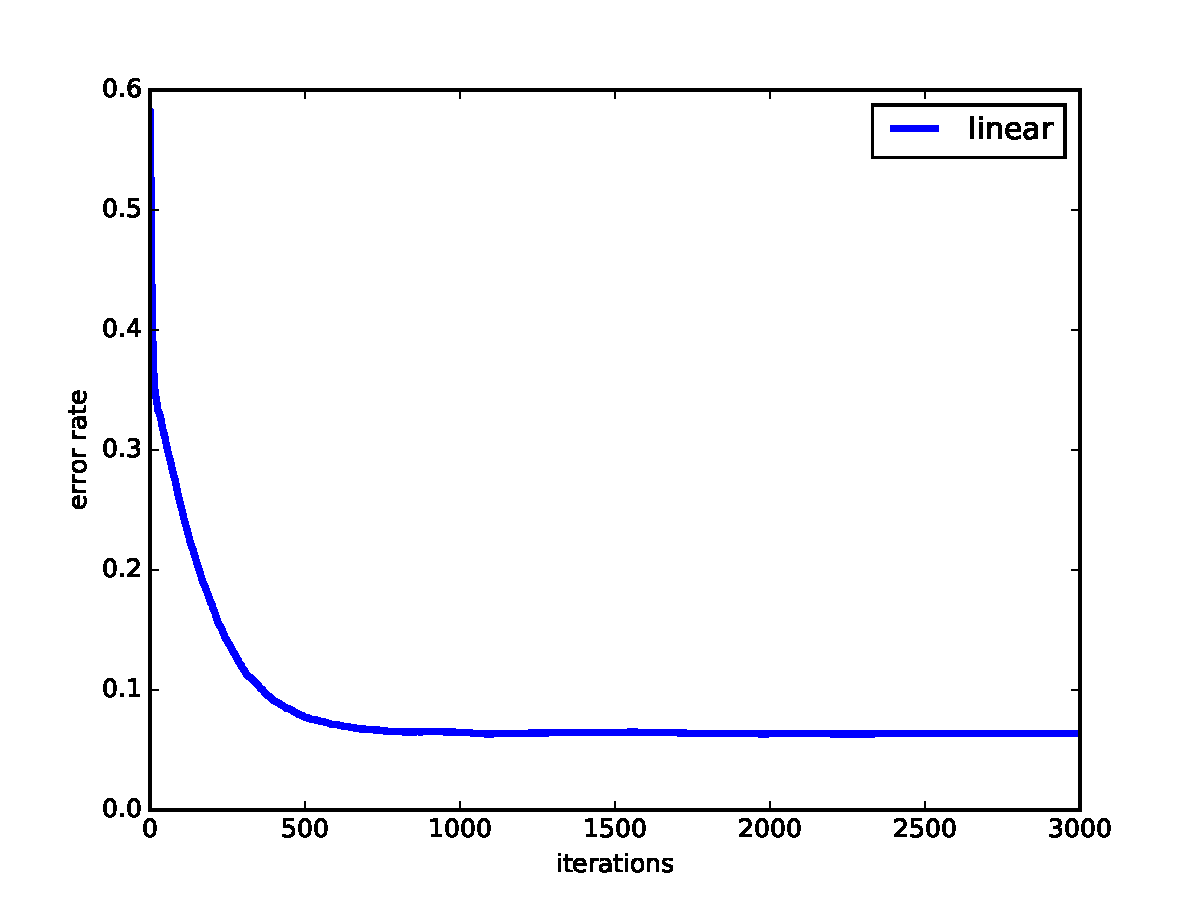
\includegraphics[width=0.45\textwidth]{../figures/part1-linear.pdf}
      }
      \subfigure[logistic]
      {
      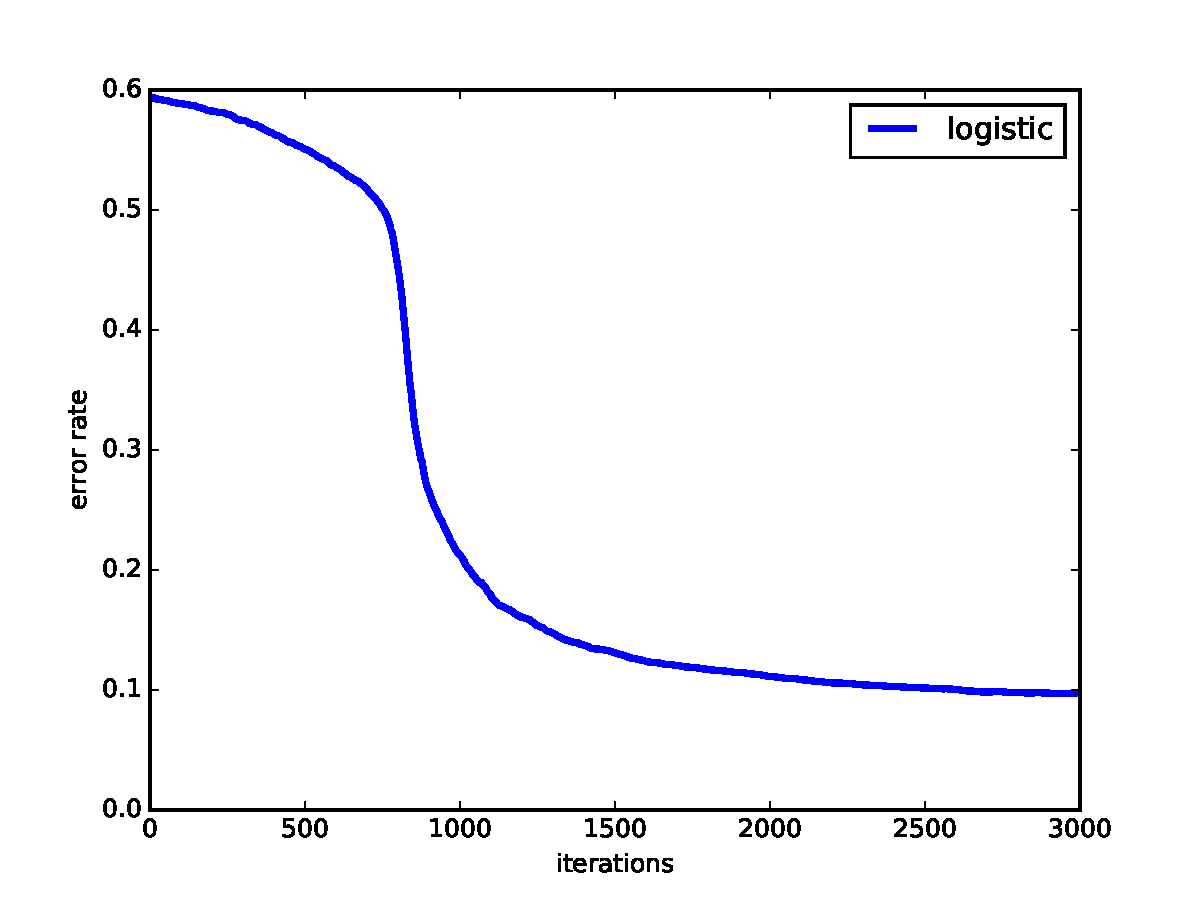
\includegraphics[width=0.45\textwidth]{../figures/part1-logistic.pdf}
      }
      \subfigure[perceptron]
      {
      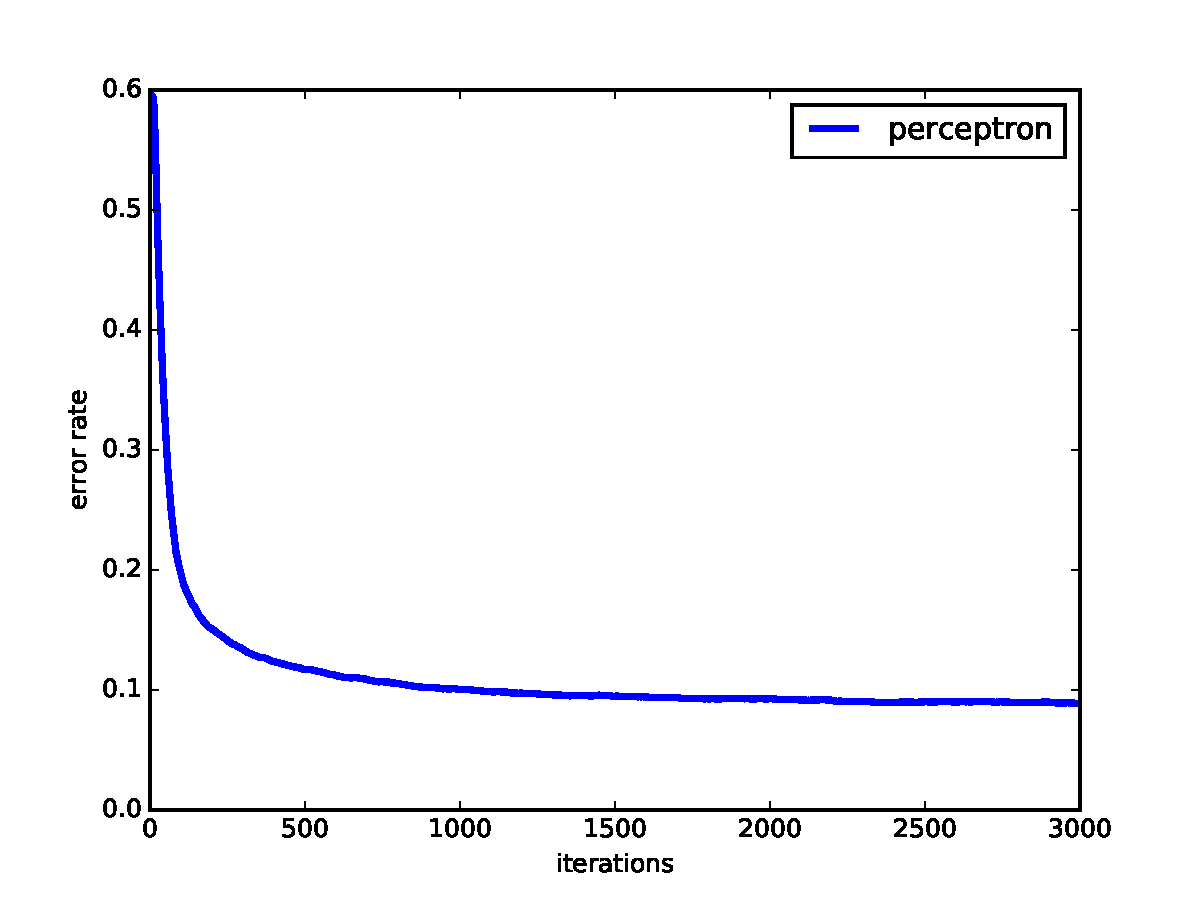
\includegraphics[width=0.45\textwidth]{../figures/part1-perceptron.pdf}
      }
      \subfigure[svm]
      {
      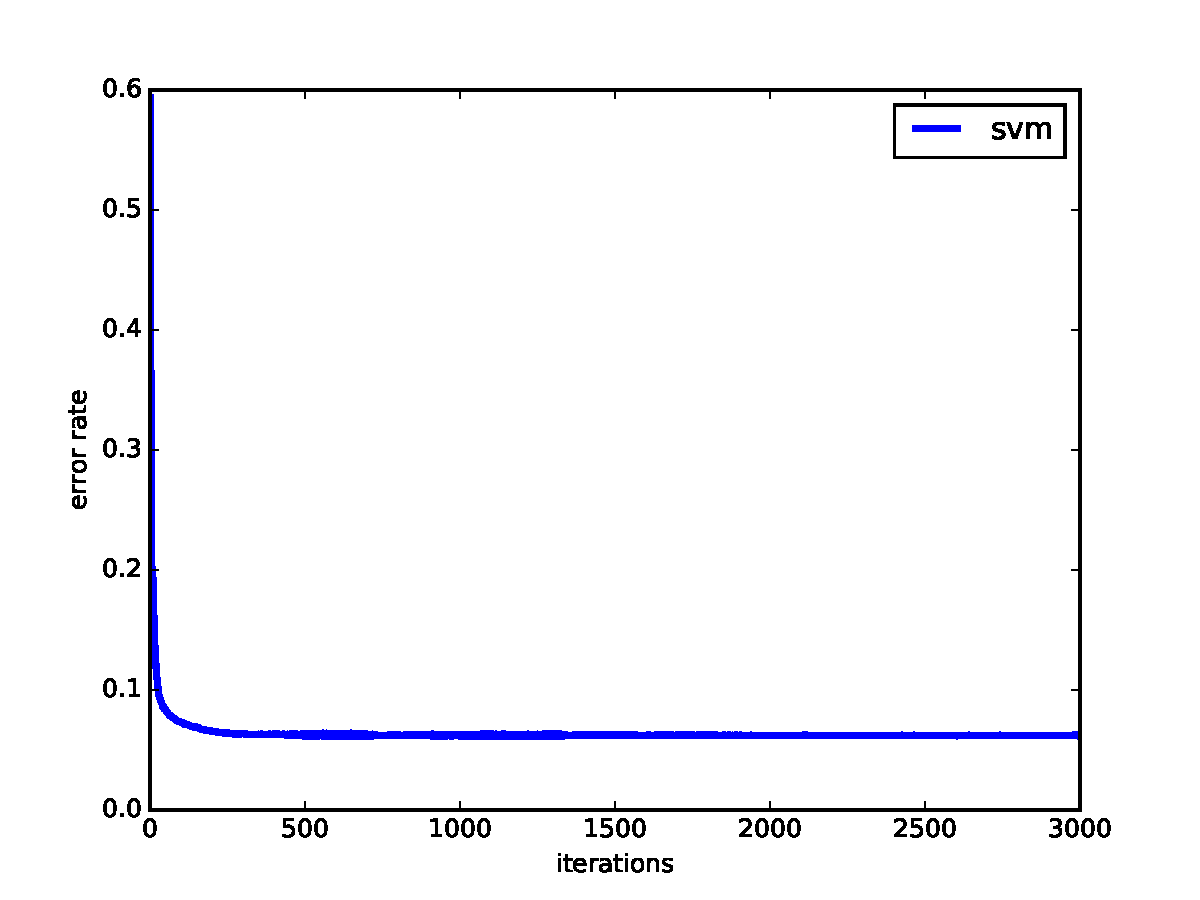
\includegraphics[width=0.45\textwidth]{../figures/part1-svm.pdf}
      }
    \end{center}
    \caption{Convergence rate of four classifiers with training step size {\rm 2e-6}.\label{fig:1}}
    \end{figure}
  \end{proof}
  \item Provide a figure, showing the training-corpus and development-test-corpus error rates of at least four different SVM training runs, using five different values of the $C$ parameter (abscissa = $C$, ordinate = error rate).
  \begin{proof}
    The plot is shown in Figure \ref{fig:2}, where we see the lowest error rate of SVM is achieved at $C=10$.
    \begin{figure}
      \begin{center}
        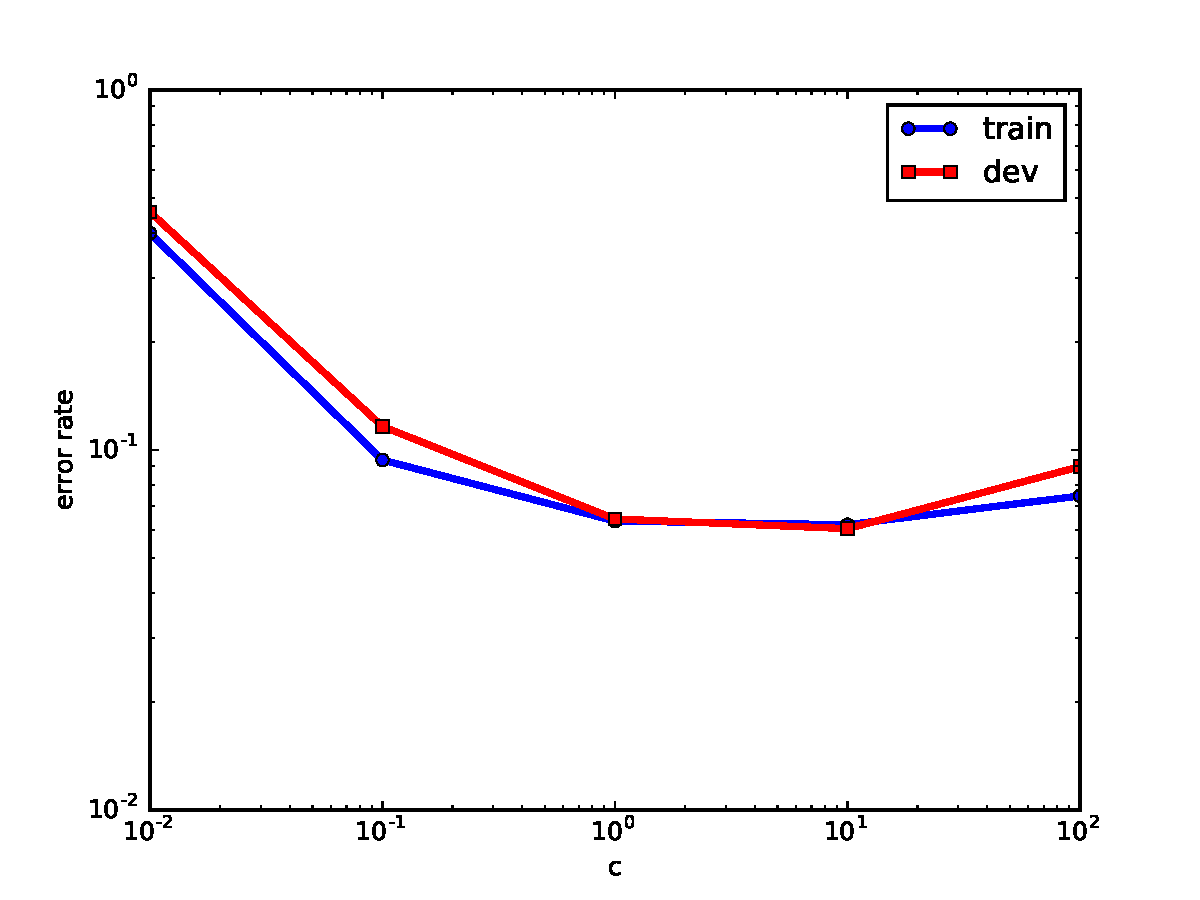
\includegraphics[width=0.45\textwidth]{../figures/part2.pdf}
        \caption{Error rate on training-corpus and development-corpus of SVM with $C$ varied from 1e-2 to 1e2.\label{fig:2}}
      \end{center}
    \end{figure}
  \end{proof}
  \item Provide a table, showing the evaluation-test-corpus error rates of all four classifiers (including whichever SVM has lowest error rate on the development-test corpus).
  \begin{proof}
    We set the step size to be 2e-6, set the number of iterations to be 3000, and set the parameter $C$ to be 10 in SVM. The resulting performances is listed in Table \ref{tb:2}.
    \begin{table}[htbp]
    \begin{center}
      \begin{tabular}{c|c}
      \hline
      {\bf classifier} & {\bf error rate(x100)} \\
      \hline
      linear & 3.5\\
      logistic & 7.1\\
      perceptron & 6.9\\
      linear SVM & 3.4\\
      \hline
      \end{tabular}
      \caption{Error rate on test set for four classifiers. \label{tb:2}}
    \end{center}
    \end{table}
  \end{proof}
  \item Provide a figure showing a scatter plot of 300 randomly selected training tokens, with 'o' used to signify ee-set and 'x' used to signify eh-set tokens, depicted in the space defined by their first two principal components, with lines drawn across the space in four different colors showing the boundary lines of the four different classifiers.
  \begin{proof}
    We use {\tt np.random.choice} to randomly generated 300 tokens from the training data, project them into two dimension using PCA. The lines are drawn accordingly in Figure \ref{fig:4}.
    \begin{figure}[htbp]
      \begin{center}
        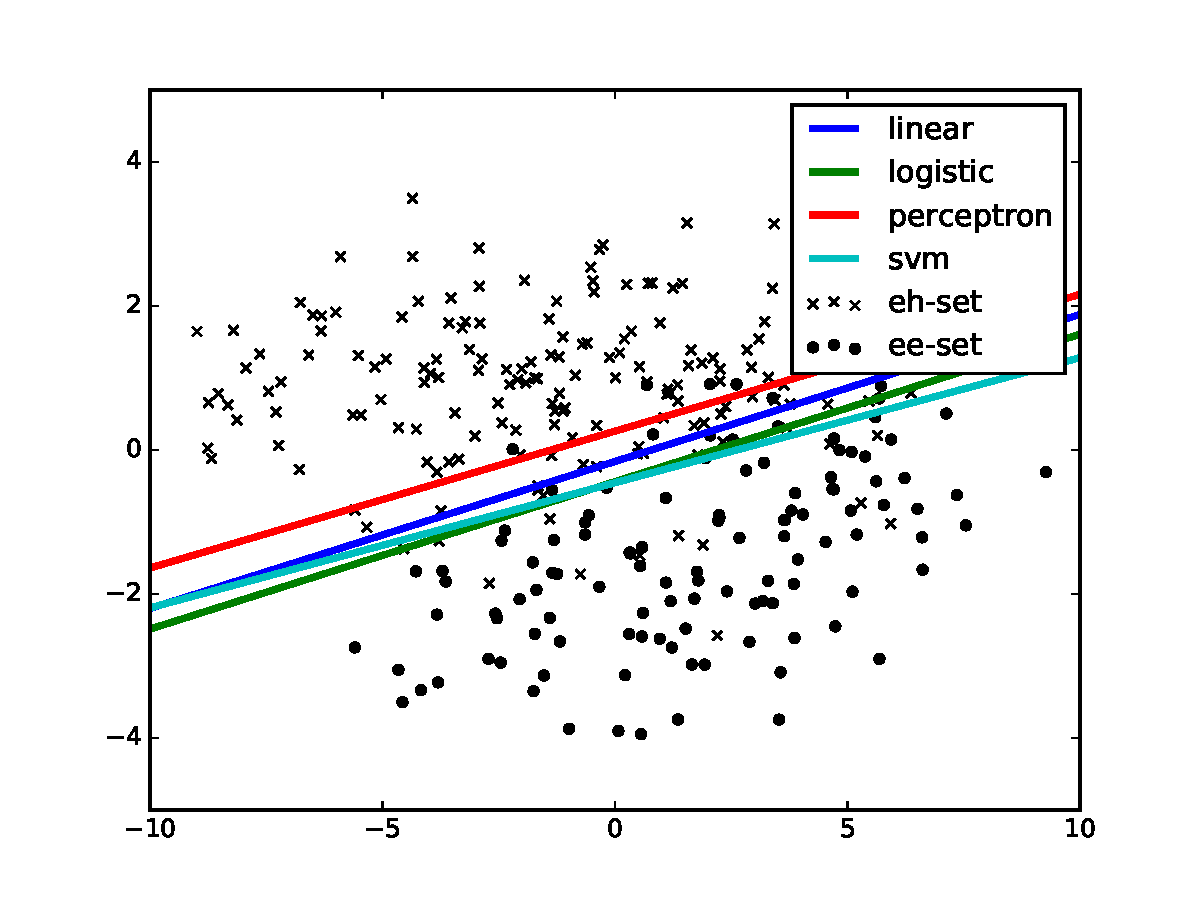
\includegraphics[width=0.45\textwidth]{../figures/part4.pdf}
        \caption{Visualization of four linear classifiers.\label{fig:4}}
      \end{center}
    \end{figure}
  \end{proof}

\end{itemize}

\section{TensorFlow}
Train a one-layer neural net, with logistic output nodes, using TensorFlow. Hint: this will be very similar to MNIST for beginners\footnote{\url{https://www.tensorflow.org/versions/r0.10/tutorials/mnist/beginners/index.html}}, but with different data. This part of the assignment should be written in Python.

Note that a logistic node is exactly equal to a two-class softmax node. Cross-entropy loss is not the same as MSE loss; you can use whichever one you prefer.

What to turn in:

\subsection{Methods}
Discuss which TensorFlow functions you used, and how.
\begin{proof}
  The functions are listed as follows:
  \begin{itemize}
    \item {\tt tf.placeholder}: is used to hold a space for some values,
    \item {\tt tf.Variable}: is used to store variables.
    \item {\tt tf.softmax}: is an implemented softmax function.
    \item {\tt tf.reduce\_mean}: computes the mean over all examples.
    \item {\tt tf.train.GradientDescentOptimizer}: is a gradient descent optimizer.
    \item {\tt tf.equal}: is to check whether two elements are equal or not.
    \item {\tt tf.argmax}: is an argmax function.
    \item {\tt tf.matmul}: is a multiplication between matrices.
    \item {\tt tf.initialize\_all\_variables}: is for initialization
    \item {\tt tf.Session}: is an interactive session.
  \end{itemize}
\end{proof}

\subsection{Results}

Provide a convergence figure (abscissa = training iteration, ordinate = training corpus error rate). Provide a table showing error rate on the training corpus, and on the evaluation-test corpus.


  \begin{figure}[htbp]
    \begin{center}
      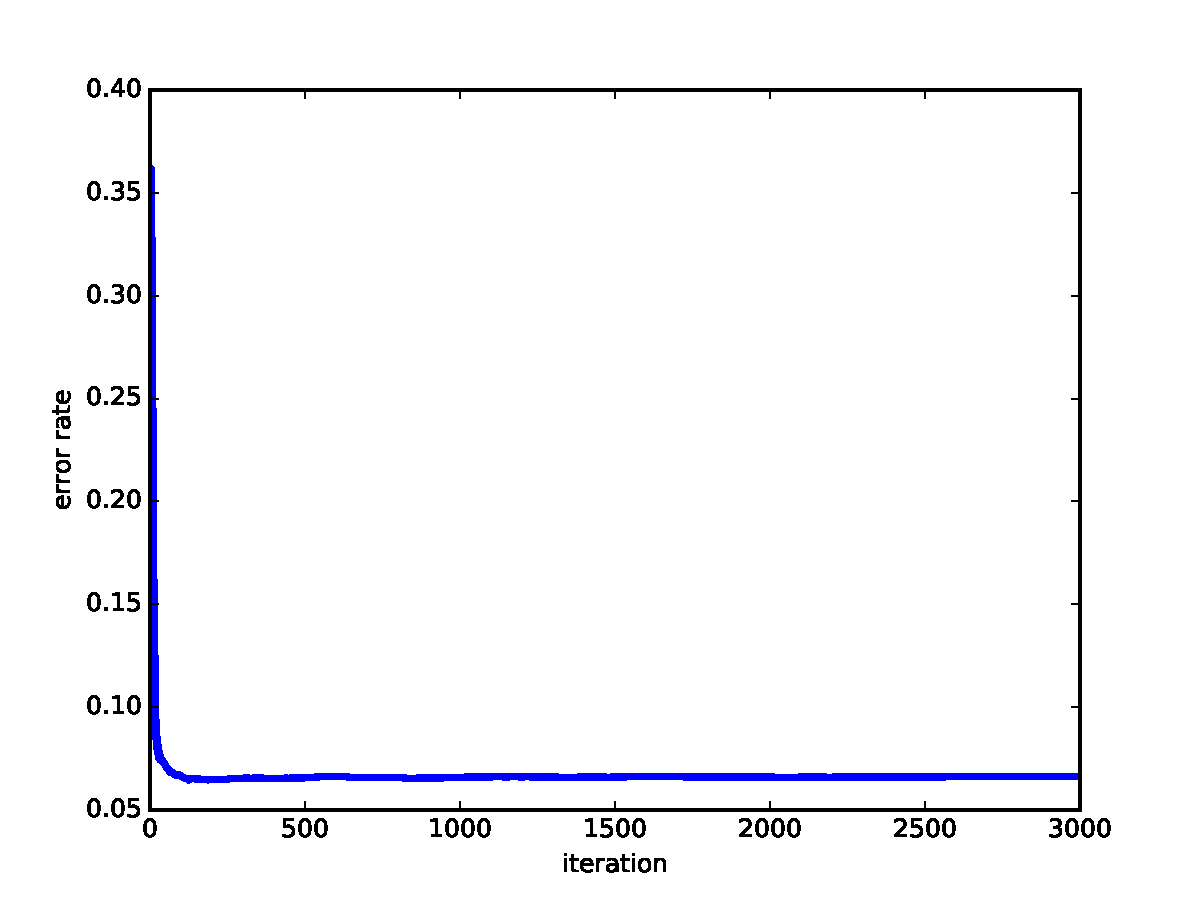
\includegraphics[width=0.45\textwidth]{../figures/tensorflow.pdf}
    \end{center}
    \caption{Convergence rate of softmax implemented by tensorflow.\label{fig:3}}
  \end{figure}

\begin{proof}
  The figure is in Figure \ref{fig:3}, where we set the step size to be 0.2. The performances on the training corpus and test corpus are reported in Table \ref{tb:3}.
\end{proof}
 \begin{table}[htbp]
    \begin{center}
      \begin{tabular}{c|c}
      \hline
      {\bf train} & {\bf test} \\
      \hline
      6.6 & 3.6\\
      \hline
      \end{tabular}
      \caption{Error rate (x100) on training set and test set for softmax classifier. \label{tb:3}}
    \end{center}
    \end{table}
\end{document}
